\documentclass[11pt, titlepage, a4paper]{article}

\usepackage{graphicx} % For images
\graphicspath{ {./graphics/} }
\usepackage[acronym]{glossaries}
\usepackage[automake]{glossaries-extra}
\usepackage[utf8]{inputenc} % For special characters
\usepackage[english]{babel} % For language-specific hyphenation patterns
\usepackage[hidelinks]{hyperref} % For clickable links
\usepackage{enumitem}
\usepackage[]{datetime2}
\usepackage[a4paper, total={15.0cm, 25cm}]{geometry}
\usepackage[backend=biber, style=ieee, sorting=none]{biblatex}
\addbibresource{Internship.bib} % Imports bibliography file+
\def\labelitemi{--}
\usepackage[T1]{fontenc}
\usepackage{inconsolata}

\usepackage{color}

\definecolor{pblue}{rgb}{0.13,0.13,1}
\definecolor{pgreen}{rgb}{0,0.5,0}
\definecolor{pred}{rgb}{0.9,0,0}
\definecolor{pgrey}{rgb}{0.46,0.45,0.48}

\usepackage{listings}
\lstset{language=Java,
  showspaces=false,
  showtabs=false,
  breaklines=true,
  showstringspaces=false,
  breakatwhitespace=true,
  commentstyle=\color{pgreen},
  keywordstyle=\color{pblue},
  stringstyle=\color{pred},
  basicstyle=\ttfamily,
  %moredelim=[il][\textcolor{pgrey}]{$$},
  moredelim=[is][\textcolor{pgrey}]{\%\%}{\%\%}
}

\title{Internship Report}
\author{Emily Sterthaus \\ Matriculation Number: 451 342 \\ \href{mailto:m_ster15@uni-muenster.de}{m\_ster15@uni-muenster.de}\\ \\
\small Ifgi Supervisor: Christian Knoth\\ \small con terra Supervisor: Thore Fechner
}
\date{\today}
\newcommand{\myparagraph}[1]{\paragraph{#1}\mbox{}\\}
\setcounter{secnumdepth}{5}
\setcounter{tocdepth}{5}
\makeglossaries
\newacronym{gd}{GD}{Geologischer Dienst}
\newacronym{exif}{EXIF}{Exchangeable Image File Format}
\newacronym{iptc}{IPTC}{IPTC Information Interchange Model}
\newacronym{csw}{CSW}{Catalogue Service for the Web }


\begin{document}


\maketitle
\newpage
\tableofcontents
\newpage

\section{Introduction}

My Internship was done at the con terra Münster. It started 2023-09-01 and ended 2024-03-31.
\subsection{Company Profile}
The con terra is a Geo IT Company Located in Münster, Germany. It developes primarily custom GeoIT Solutions, based on the Feature Manipulation Engine (FME) and various Esri Technologies, such as ArcGIS. Therefore the con terra is Esri Platinum Partner and the main distribution Partner from Safe Software for FME.

Based on this, the con terra also provides their own products, such as map.apps and smart.finder. Each with multiple different addons and configurations, for example smart.finder - SDI or map.apps ETL. Their also working on a open source Framework as an alternative, called Open Pioneer.   %Todo: Hierüber muss ich drignend mit thore sprechen ob das so passt

The con terra works with multiple different company and governmental Organizations, such as TenneT TSO,  \glsxtrfull {gd} NRW, IT.NRW or the Bundesanstalt für Geowissenschaften und Rohstoffe  (BGR).

\subsection{Motivation}

%Todo: Irgendeine begrüdung finden die weder geld noch "kenn ich schon" ist 

\section{Internship Content}

My internship was clearly structured. This took the form three different Projects, each in their own timeframe and with their own requirements.

\subsection{Geologischer Dienst NRW - Metdata Asset Managment System}
\subsubsection{Introduction}
The  \glsxtrshort {gd} NRW has a large achieve of different assets, which are currently managed by a software named cumulus. As the used software is outdated, it does not meet the the current requirements.
Primarily they  are required to make all data, where it is legally possible, open data \cite{GesetzZurForderung2017}.
Additionally the GeolDG also requires the \glsxtrshort{gd} to make their accessible by the public \cite{GesetzZurStaatlichen2020}.

Therefore the main goal of this project was to conceptualize a new system and to implement parallel a prototype of it.
\subsubsection{As-is Status}
The digital archive of the  \glsxtrshort{gd} consists of over 450 thousand Assets. Assets in this context are for example Images, PDFs, TIFs or MP4s. But each digital file can be an asset. The total data volume is over 2 Terrabyte.
These assets are currently on a shared drive and can be managed via the filesystem. Additionally they use a software called Cumulus. This software manages primarily the associated asset metadata. Currently the \glsxtrshort{gd} does not use any well known Metadata schema, instead they use a list of custom attributes, e.g. Rating, Special Instructions and Label.
Additionally they use \glsxtrshort{exif} and \glsxtrshort{iptc} Metadata Information for Images, which is not managed by the Cumulus. Instead it its done with an additional software component. %Likely Irfanview 

\subsubsection{The new system}
The new system exists maninly as a concept. But a few features were already implemented as a prototype for the \glsxtrshort{gd} to test them.
\myparagraph{Requirements}
The new system should eliminate the inadequacies of the old system. Therefore a list of Requirements were collected. In the following there is a subset example of the main functional requirements:
\begin{itemize}
	\item Keeping the Internal metadata attributes (and adding new ones)
	\item Connection to the GEOportal.NRW
	\item CRUD Operations for Datasets and associated metadata
	      \begin{itemize}
		      \item With an Integrated Permission System for Internal (\glsxtrshort{gd} Employees) and Externals
		      \item Multi-Edit for Metadata
	      \end{itemize}
	\item Sharing data
	\item Update \glsxtrshort{exif} and \glsxtrshort{iptc} when an update occurs
	\item Syncing/Translating Internal Metadata to ISO 19115/ISO 19119
	\item Different Search Operations
\end{itemize}


\begin{figure}[t]
	\caption{Use case diagram, which visualized a some functional requirements}
	\label{fig:usecase}
	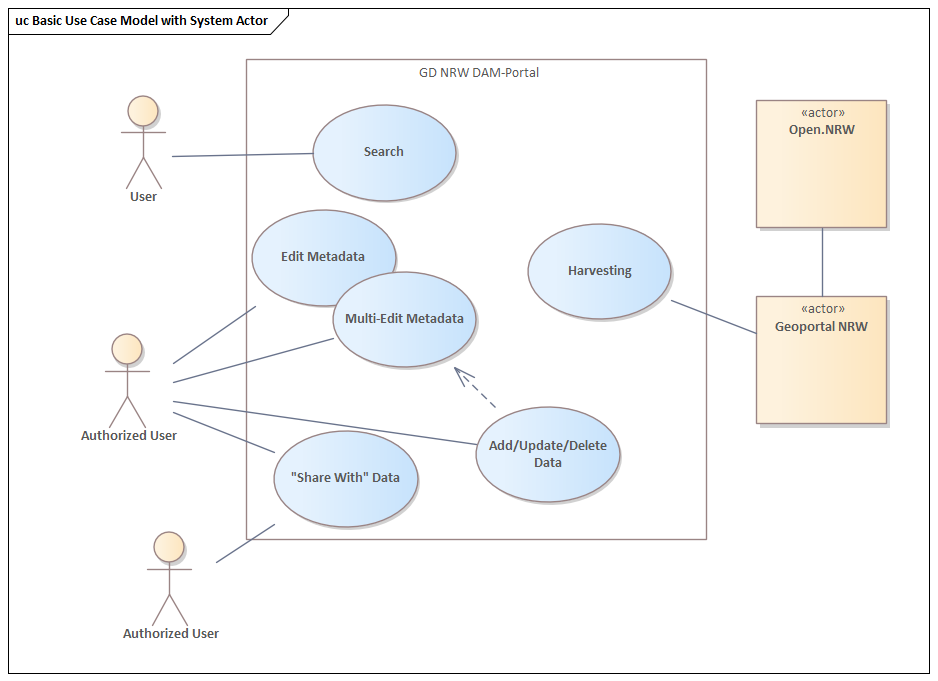
\includegraphics[width=16cm]{usecase_diagramm.png}
	\centering
\end{figure}


Additionally there are a few Quality Requirements, primarily focusing on data integrity and the used techstack for the developement. For example the developed software should be able to live in the cloud or in dedicated Machine.

One final requirement is that the system needs to be splitted. It should run mainly on the servers from IT.NRW. But only non-sensitive data should be on hosted by them. Sensitive data should  be hosted and only accessible by the \glsxtrshort{gd} and its associates. 

\myparagraph{Implementation}
To meet these new Requirements the smart.finder SDI was choosen as base software. As it can not meet all requirements standalone (for example it can only work with ISO 19115/ISO 19119, INPSIRE or GDI DE Metadata) new software components were conceptualized and implemented to meet the designated requirements.

\begin{figure}[t]
	\caption{Planned software components (partial abstracted)}
	\label{fig:components}
	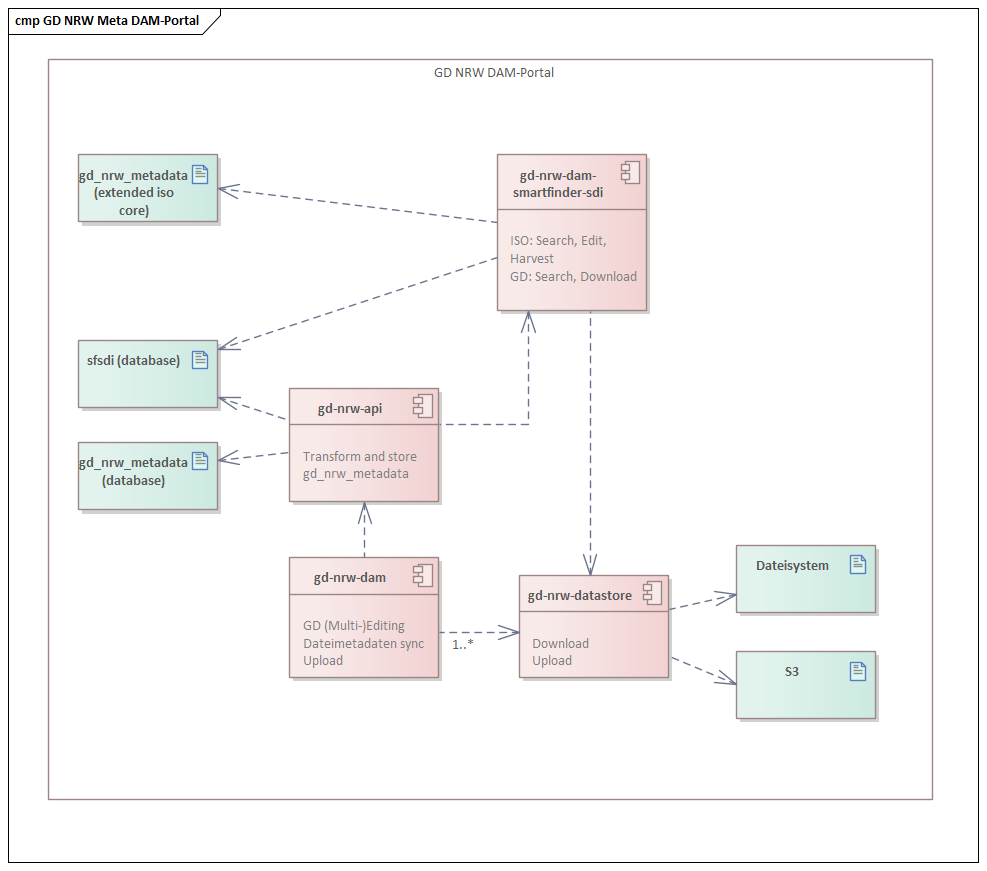
\includegraphics[width=16cm]{components.png}
	\centering
\end{figure}

As seen in \ref{fig:components} the new Software consists of a gd-nrw-api, gd-nrw-dam-smartfinder-sdi, gd-nrw-dam and gd-nrw-datastore.
In the following each software component will be shortly described:
\begin{description}[]
	\item[gd-nrw-dam-smartfinder-sdi]: This represents the smart.finder sdi. itself consits of multiple software components, such as the smartfinder-search, smartfinder-editor, smartfinder-csw and the smartfinder-sdi, and the gd-nrw-dam-portal.
	      \begin{description}[]
		      \item[smartfinder-search]: This component manages primarily the data handling. It operates on an integrated Apache Solr instance to enable the search and filter capabilites of the smartfinder. It also allows aspects like full-text search, geo-searches or filter for specific attribute values.
		      \item[smartfinder-editor]: This component represents the smart.editor. It allows editing Metadata which complys to with ISO 19115/ISO 19119, INPSIRE or GDI DE.
		      \item[smartfinder-csw]: This component is the \glsxtrshort{csw} -interface. It allows sharing data to other portals, such as the GEOportal.NRW.
		      \item[smartfinder-sdi]: This component thereby represents the frontend used for search and viewing datasets.
		      \item[gd-nrw-dam-portal]: This component is an adapted version of the smartfinder-sdi component.
	      \end{description}
	\item[gd-nrw-dam]: This component provides  CRUD functionality of metadata. Especially it provides an frontend for Multi-Edit Metadata, Editing Single Metadata,
	\item[gd-nrw-datastore]: This component handles data raw data access. It can either work with the raw file system or S3 Storages. It provides basic CRUD capabilites for the data.
	\item[gd-nrw-api]: This component handles the interaction between the new developed software components and the smartfinder-sdi.
\end{description}
The general workflow for documents is that all editing is handled from gd-nrw-dam. The edits then will be synchronized to the smartfinder-sdi.
To save these \glsxtrshort{gd} specific attributes, there is also a new database, called gd-nrw-metadata.

\begin{figure}[t]
	\caption{Deployment Diagramm}
	\label{fig:deployment}
	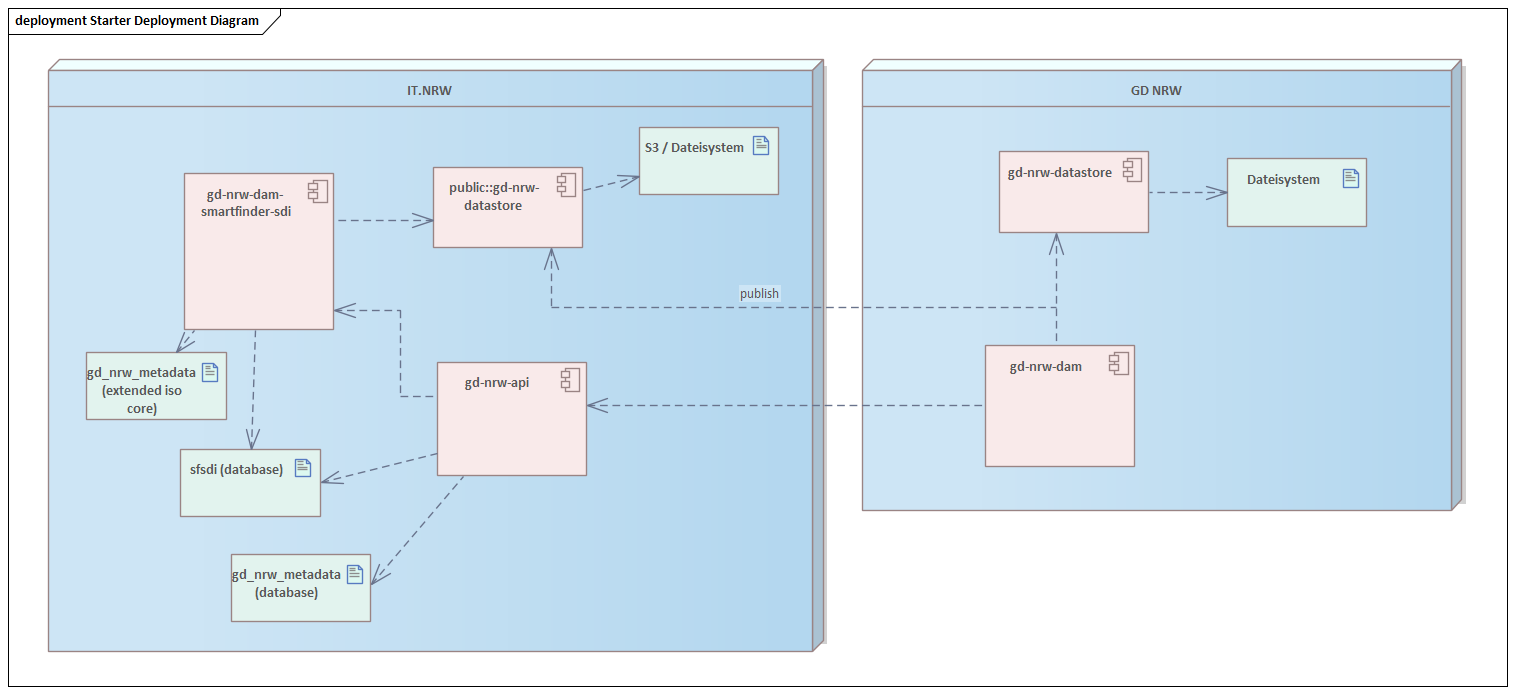
\includegraphics[width=16cm]{deployment.png}
	\centering
\end{figure}

To meet the requirement regarding the hosting of sensitive data, a deployment diagramm was created \ref{fig:deployment}. To achieve the goal there are now two datastores which can be inplace switched. This is necessary to give authorized users access to sensitive data. The metadata in this case is still completely hosted by IT.NRW but may be locked behind an login and is therefore not available by the public. The aim of this configuration is to duplicate as few services as possible.
An alternative was to build complete clone system for IT.NRW and \glsxtrshort{gd} and only synchronize the open access datasets.

\subsubsection{My Participation}
My participation in this project was primarily the developement of the new software components for a prototype. Additionally i made modified the smartfinder-sdi. 

\begin{figure}[t]
	\caption{Database Scheme}
	\label{fig:db}
	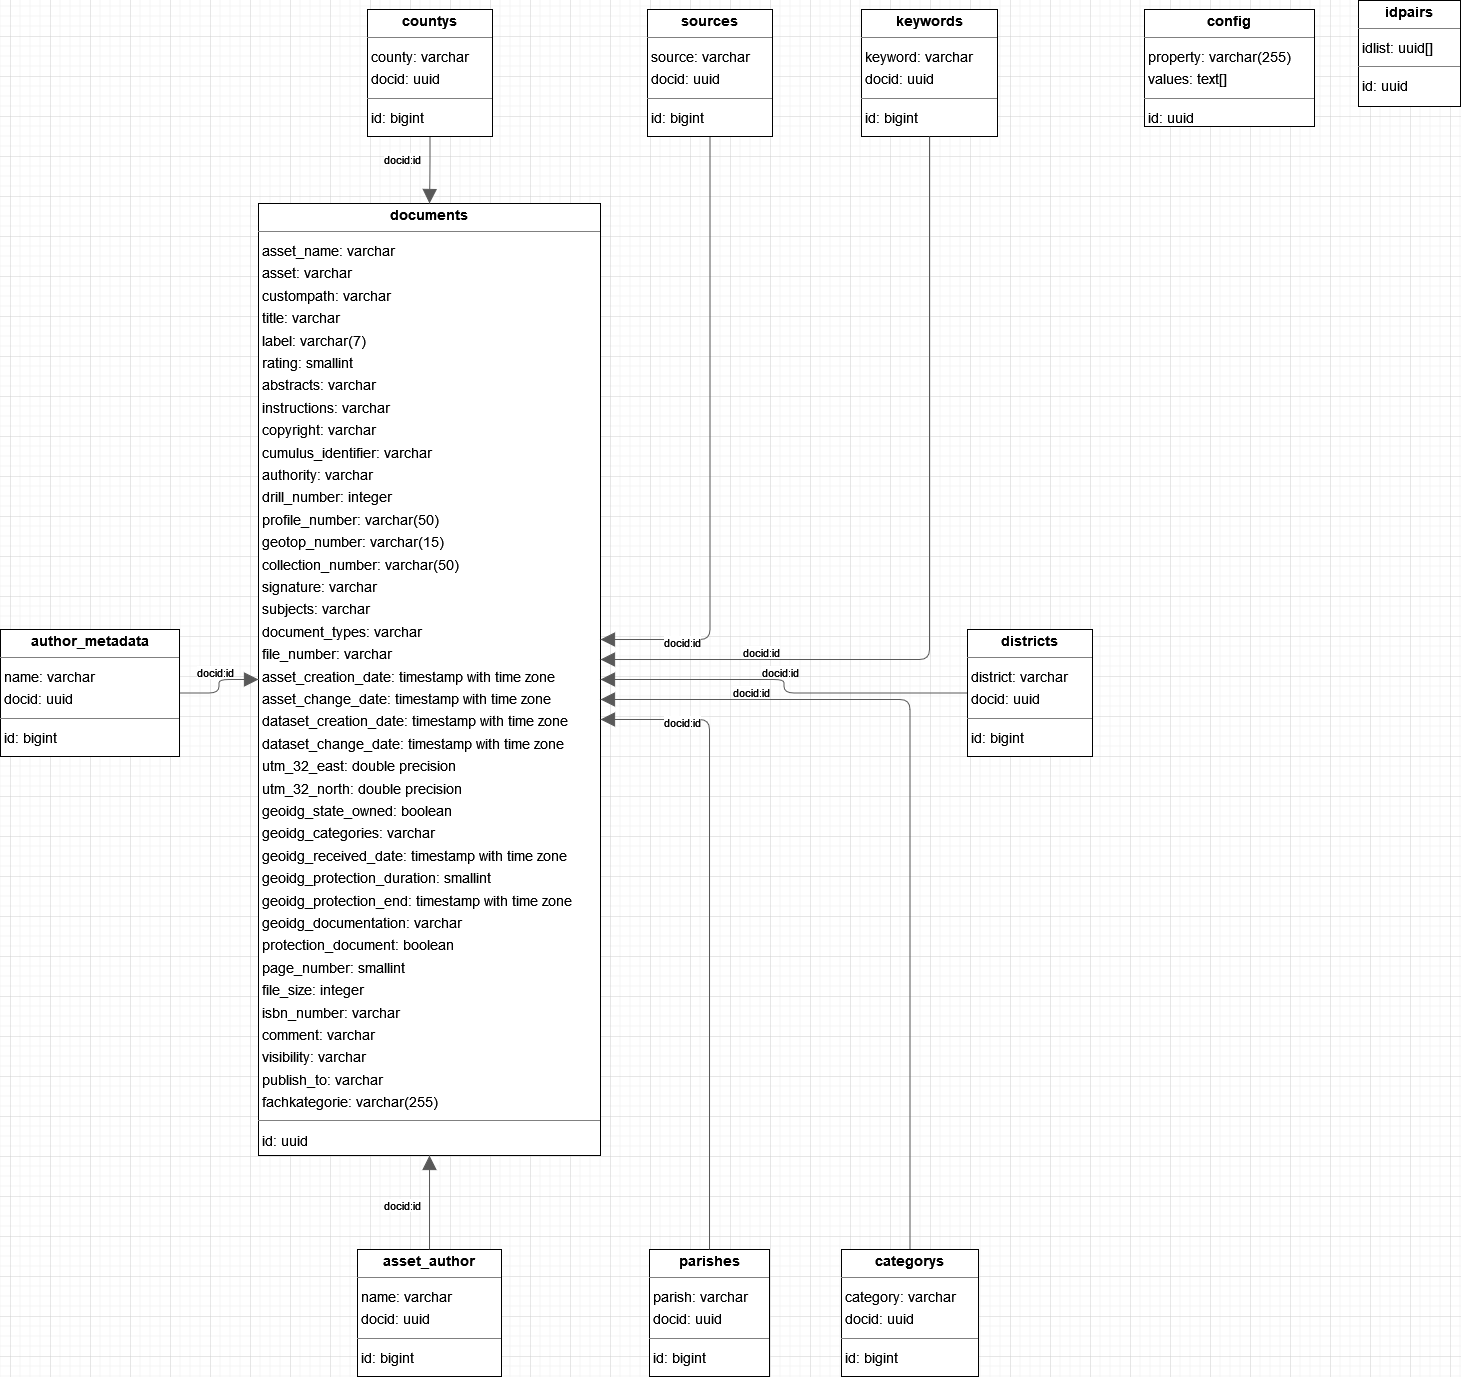
\includegraphics[width=16cm]{db3.png}
	\centering
\end{figure}

The first prototype started as a simple project based on FastAPI and Python. With a addtional PostgreSQL database. Primarily the focus at this time was to develope a database schema which fullfills our needs. The final scheme is visible in Graphic \ref{fig:db}. It was choosen to use a flat structure without N-M relationships. 
Also the first version for the frontend was developed by me. As a tech stack it was choosen to use Vue and Vuetify, with a Vite developement server. The main vue components i developed were a Single Editing, for editing a single Metadaset, and a Multi-Edit for editing an arbitrary number, greater 1, of Metadatasets. For the single editing i became later on a Mockup as a template, on which it is based. The Multi-Editing was meanwhile designed and conceptualized by me, as seen in \ref{fig:multiedit}. 

\begin{figure}[t]
	\caption{Screenshot MultiEditing}
	\label{fig:multiedit}
	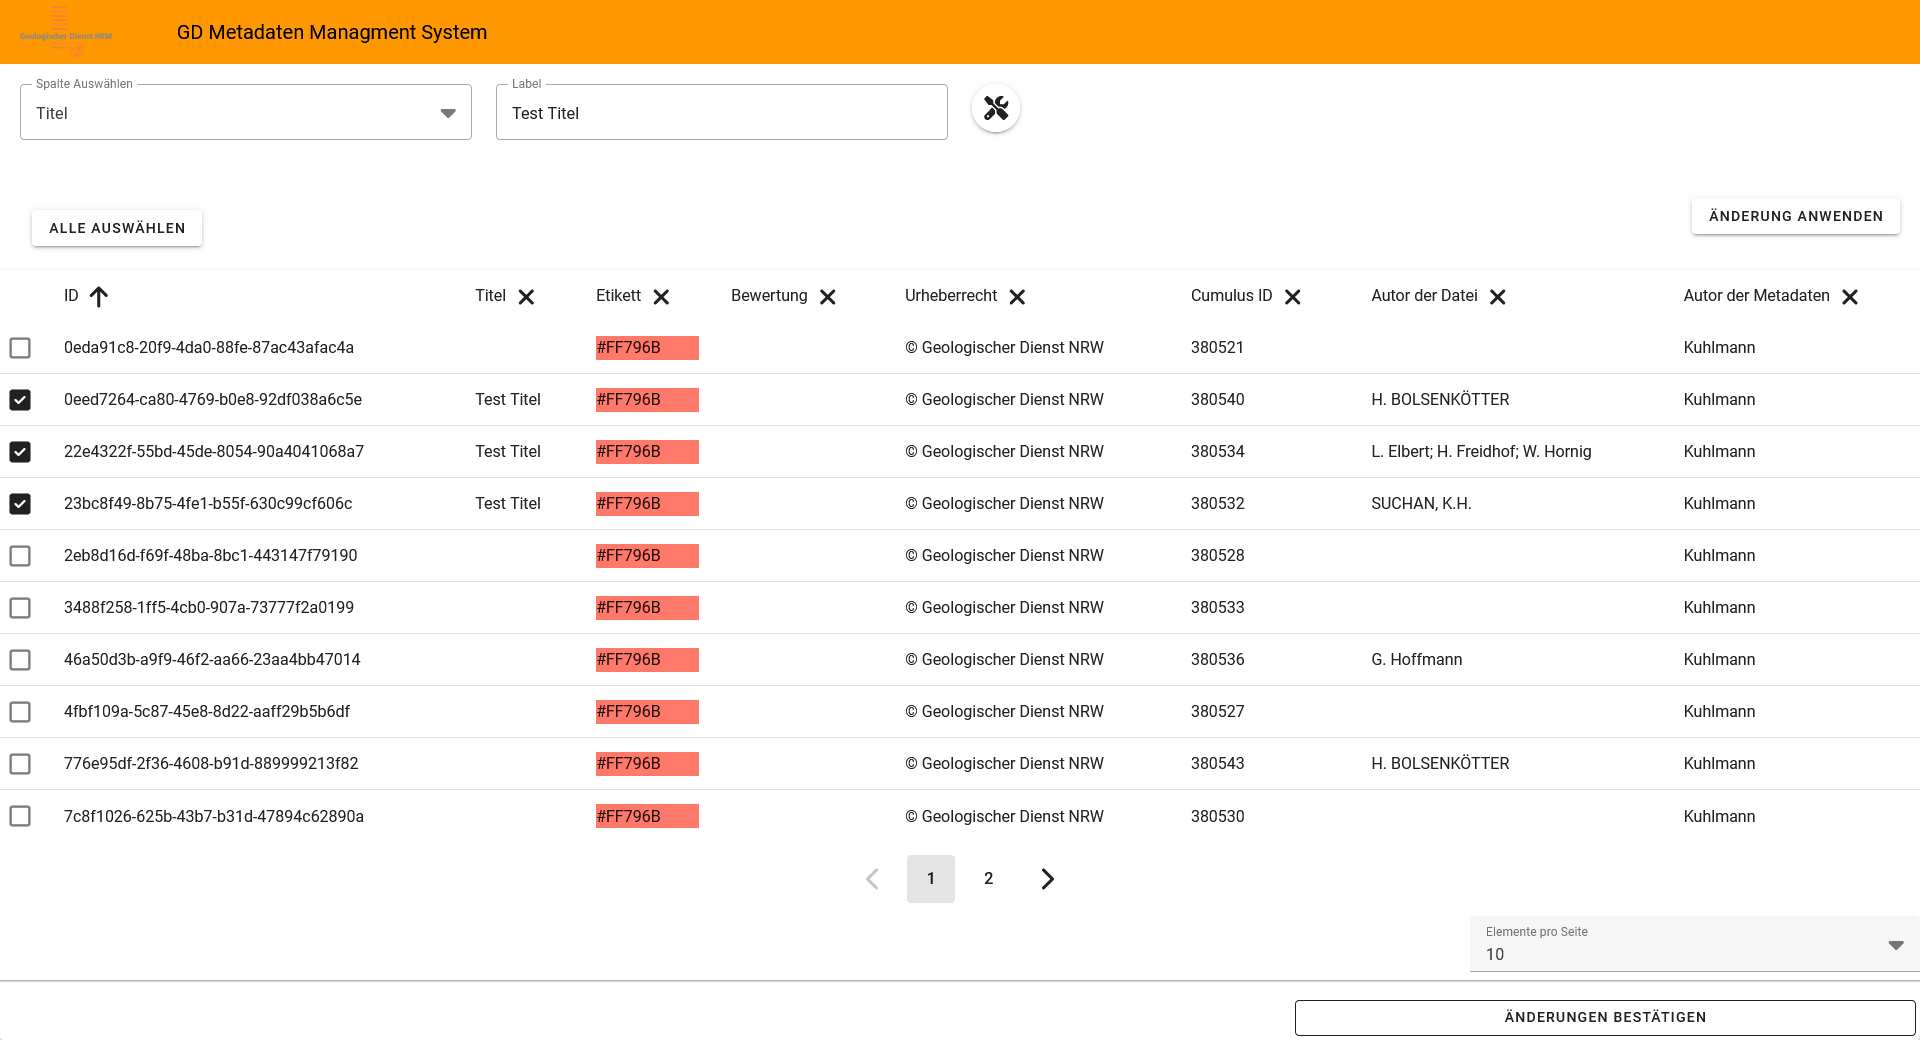
\includegraphics[width=16cm]{multiedit.png}
	\centering
\end{figure}
\begin{figure}[t]
	\caption{Vue Controller}
	\label{fig:vue}
	\begin{lstlisting}[language=java]
        @Controller
        public class VueController {
            @RequestMapping(value = "/*/{path:[^\\.]*}")
            public String redirect(){
                return "forward:/";
            }
        
        
        }
        
        \end{lstlisting}
	\centering
\end{figure}


After that it was quickly decided to drop Python and FastAPI in favor of Spring Boot and Java. Therefore i started to write the gd-nrw-dam component, which is currently gd-nrw-datastore component. It started with implementing the necessary spring data classes and interfaces. After that i started implementing the basic endpoints for updates, to regain functionality for my frontend. Also i added the capabilites to host the build frontend by the spring boot server. For that i wrote a Spring Boot special controller to keep the Vue Router Component from the frontend working, as it controls the routing for which page is loaded. 






\subsection{Digitaler Zwilling - Fire Department Live Data}
\subsection{Open Pioneer - TBA}
\section{Reflection}

\clearpage
\printglossary[type=\acronymtype]
\printglossary
\clearpage
\printbibliography

\end{document}
